
\documentclass{scrartcl}
\usepackage{tikz}
\usetikzlibrary{arrows,automata}

\begin{document}
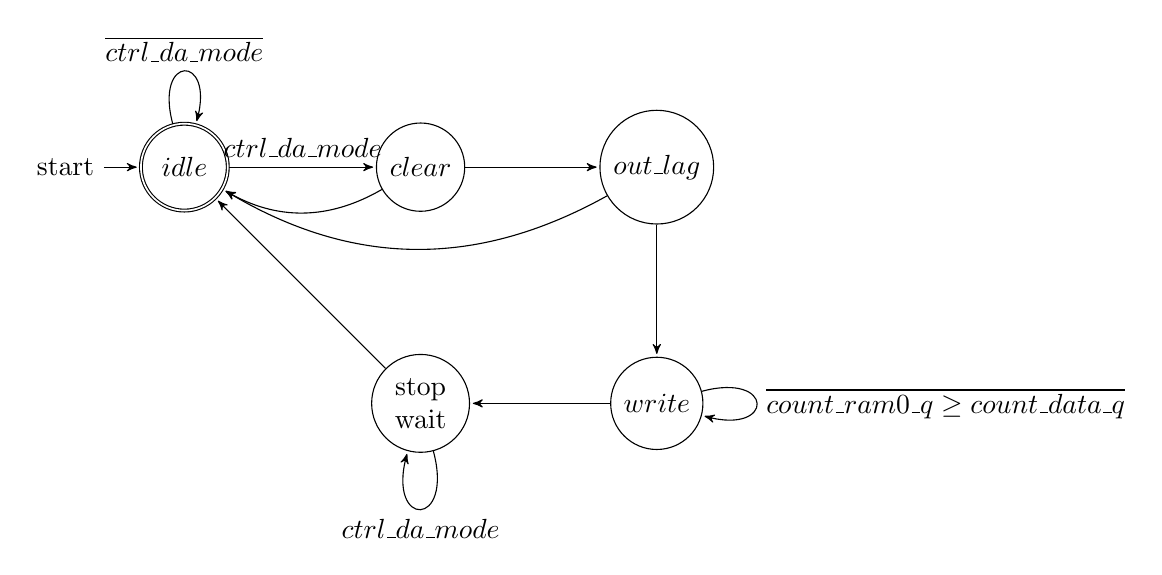
\begin{tikzpicture}[>=stealth',shorten >=1pt,auto,node distance=3cm]
  \node[initial,state,accepting, inner sep=5pt] (idle)         {$idle$};
  \node[state]                   (clear) [right of=idle]       {$clear$};
  \node[state]                   (outputlag) [right of=clear]  {$out\_lag$};
  \node[state]                   (write)  [below of=outputlag] {$write$};
  \node[state, align=center]     (stopwait)  [left of=write] {stop\\wait};

  \path[->]
  (idle)
  edge [loop above]
  node 
  {$\overline{ctrl\_da\_mode}$} (idle)
  edge
  node 
  {$ctrl\_da\_mode$} (clear)

  (clear)
  edge 
  node
  {} (outputlag)
  edge [bend left, pos=0.5]
  node
  {} (idle)

  (outputlag)
  edge [bend left, pos=0.4]
  node
  {} (idle)
  edge 
  node
  {} (write)

  (write)
  edge [loop right]
  node
  {$\overline{count\_ram0\_q \geq count\_data\_q}$} (write)
  edge [pos=0.3]
  node 
  {} (stopwait)

  (stopwait)
  edge 
  node 
  {} (idle)
  edge [loop below]
  node 
  {$ctrl\_da\_mode$} (stopwait)
;
\end{tikzpicture}

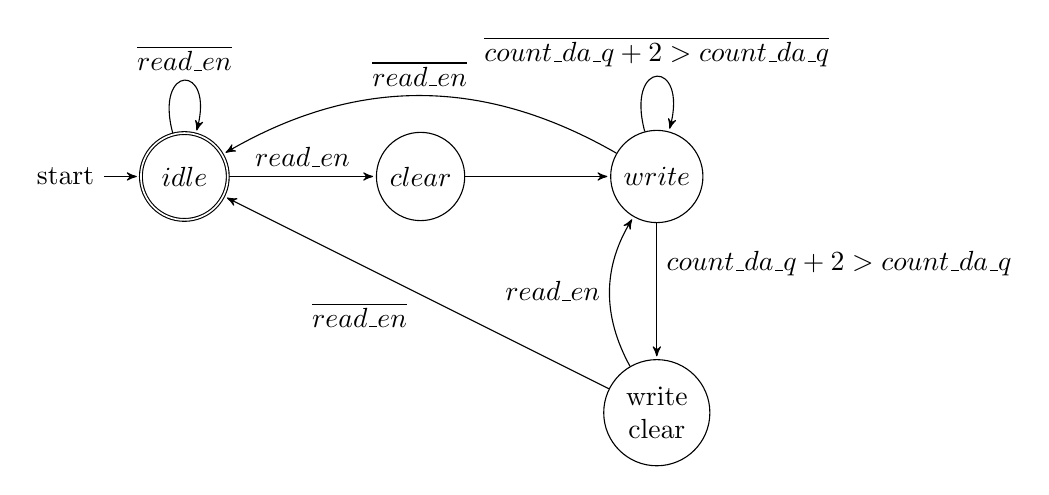
\begin{tikzpicture}[>=stealth',shorten >=1pt,auto,node distance=3cm]
  \node[initial,state,accepting, inner sep=5pt] (idle)         {$idle$};
  \node[state]                   (clear) [right of=idle]       {$clear$};
  \node[state]                   (write) [right of=clear]       {$write$};
  \node[state, align=center]     (writeclear)  [below of=write] {write\\clear};

  \path[->]
  (idle)
  edge [loop above]
  node 
  {$\overline{read\_en}$} (idle)
  edge
  node 
  {$read\_en$} (clear)

  (clear)
  edge 
  node
  {} (write)

  (write)
  edge [loop above]
  node
  {$\overline{count\_da\_q + 2 > count\_da\_q}$} (write)
  edge [pos=0.3]
  node 
  {$count\_da\_q + 2 > count\_da\_q$} (writeclear)
  edge [bend right, above]
  node 
  {$\overline{read\_en}$} (idle)

  (writeclear)
  edge 
  node
  {$\overline{read\_en}$} (idle)
  edge [bend left]
  node
  {$read\_en$} (write)

;
\end{tikzpicture}


\end{document}
